% Provenance (never printed): old terminale S material on mountain ranges and
% continental collision (folds, reverse faults and nappes as signs of
% shortening and thickening; ophiolites and sutures as the trace of a closed
% ocean; the Himalaya and the Alps as examples). Owner (Sync 0): collision,
% fold/anticline/syncline/fold axis, reverse fault/thrust, nappe, ophiolite,
% suture, shortening. Fault is Book 1's (g7), normal fault g11.05's, the root
% and Airy isostasy g11.03's and g12.01's: recalled, never redefined. India's
% past latitudes: figdata/grade-12/india_drift.py (GPlates Web Service, two
% published plate models); shortening: figdata/grade-12/fold_shortening.py;
% the belt map: figdata/grade-12/alpine_belt.py.
\chapter{La formación de las montañas}\label{ch:g12:mountain-building}

Los escaladores que llegan a la cima del Everest, a \qty{8848.86}{m} sobre el
nivel del mar, pisan caliza. Los geólogos que bajaron muestras de la cumbre
encontraron en ellas fragmentos de trilobites, ostrácodos y crinoideos:
animales marinos que vivieron hace más de 440 millones de años, en el
Ordovícico. La roca más alta del mundo se depositó en el fondo de un mar.
Este capítulo explica cómo un fondo marino acaba en el techo del mundo: dos
continentes chocan, y la corteza que hay entre ellos se comprime, se pliega,
se apila y se engrosa hasta formar una cordillera.
% ledger: sakai05:summit, tulane:roots (marine limestones at the top of Mt. Everest), ics:base.Ordovician, ics:base.Silurian (486.85-443.1 Ma); Book 1: tht:everest (8848.86 m)

\begin{omfigure}
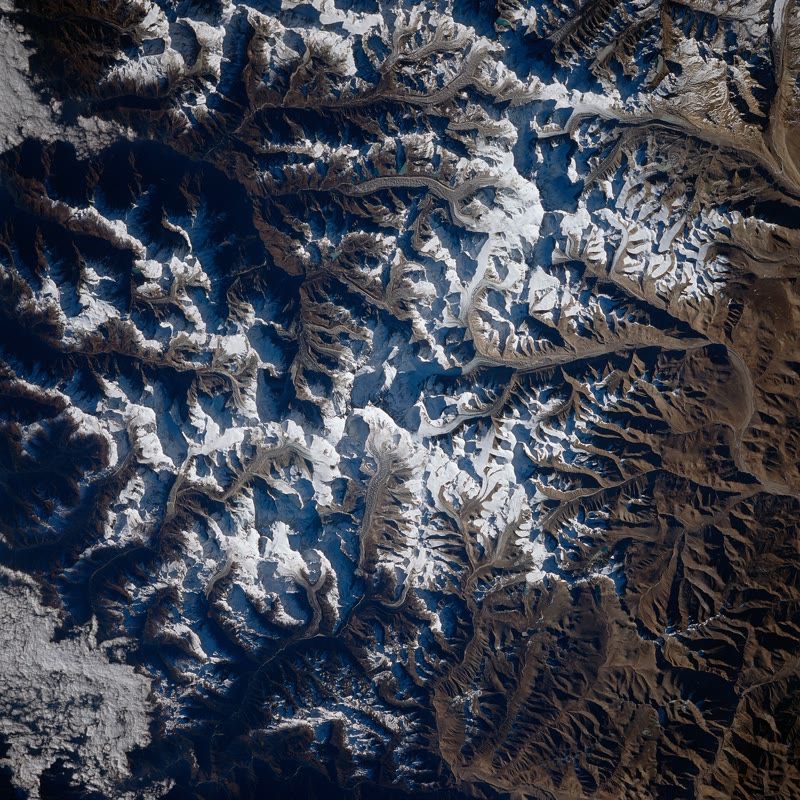
\includegraphics[width=0.5\linewidth]{images/book2/g12-nasa-everest-columbia.jpg}

{\small El Everest y muchos glaciares a su alrededor, vistos desde el
transbordador espacial Columbia el 30 de noviembre de 1996. Fotografía de la
NASA (dominio público).}
\end{omfigure}
% ledger: photo:g12-everest-columbia

\begin{recall}
Una placa de \omterm{def:g11:ocean-ridges:oceanic-lithosphere}{litosfera oceánica}, formada en una dorsal, se hunde de nuevo en
el manto en una fosa; su \omterm{def:g11:subduction-zones:slab}{losa} tira de ella hacia abajo (el
\cref{ch:g11:subduction-zones}). La \omterm{def:g12:continental-crust:continental-crust}{corteza continental} es gruesa y ligera,
de unos \qty{2830}{kg/m^3} de media frente a \qty{3380}{kg/m^3} del manto que
tiene debajo, así que flota alta, y una corteza gruesa se eleva más que una
delgada, sobre una \omterm{def:g12:continental-crust:root}{raíz}
(\cref{ch:g12:continental-crust,ch:g11:lithosphere-asthenosphere}). Una falla
es una rotura a lo largo de la cual los dos bloques se han desplazado; en una
\omterm{def:g11:ocean-ridges:normal-fault}{falla normal}, el bloque situado por encima del plano de falla ha bajado, como
donde la corteza se estira en una dorsal lenta (el \cref{ch:g11:ocean-ridges}).
\end{recall}
% ledger: cm95:crust, data:prem, tulane:no-subduct, usgs:normal-fault

\section{De la subducción a la colisión}

Un océano que se consume en una fosa más deprisa de lo que se forma en su
dorsal se encoge. Un continente que viaja sobre la placa que se hunde se
acerca a la fosa a la velocidad de la placa, y al final llega a ella. La
\omterm{def:g11:ocean-ridges:oceanic-lithosphere}{litosfera oceánica} que lo precedía se ha hundido; el continente no puede
seguirla, porque su corteza es demasiado ligera para hundirse en el manto,
más denso. La \omterm{def:g11:subduction-zones:subduction}{subducción} se detiene. Los dos continentes quedan comprimidos
uno contra otro, y la \omterm{def:g11:subduction-zones:slab}{losa} que colgaba del fondo oceánico acaba por romperse y
hundirse en el manto.
% ledger: earle:collision, tulane:no-subduct

\begin{definition}[Colisión continental]\label{def:g12:mountain-building:collision}
Una \emph{colisión continental}\index{colision continental@colisión continental} es el
encuentro de dos continentes en un límite de placas convergente, una vez
subducida la \omterm{def:g11:ocean-ridges:oceanic-lithosphere}{litosfera oceánica} que los separaba. Ninguno de los dos
continentes se hunde: la corteza que hay entre ellos se deforma y se engrosa
hasta formar un cinturón montañoso.
\end{definition}
% ledger: earle:collision, tulane:no-subduct, usgs:himalaya-collision

\begin{omfigure}
\begin{tikzpicture}[x=0.95cm, y=0.95cm, font=\scriptsize]
  % ---- stage 1: the ocean closes ----
  \begin{scope}[yshift=0cm]
    \fill[omSea] (3.4,0) -- (8.6,0) -- (8.0,-0.5) -- (4.3,-0.5) -- (3.5,0.0) -- cycle;
    \fill[omLithGranite] (0,0.15) -- (3.5,0.15) -- (4.3,-0.5) -- (4.3,-0.75) -- (3.5,-1.0) -- (0,-1.0) -- cycle;
    \fill[omLithBasalt] (4.3,-0.5) -- (8.0,-0.5) .. controls (9.0,-0.75) and (9.6,-1.2) .. (10.4,-2.0)
      -- (10.15,-2.15) .. controls (9.4,-1.4) and (8.9,-1.0) .. (8.0,-0.75) -- (4.3,-0.75) -- cycle;
    \fill[omLithGranite] (8.0,-0.5) -- (8.6,0.2) -- (12,0.2) -- (12,-1.05) -- (9.5,-1.05)
      .. controls (9.0,-0.75) .. (8.0,-0.5) -- cycle;
    \fill[omThm!70] (10.0,0.2) -- (10.3,0.55) -- (10.6,0.2) -- cycle;
    \draw[black!60, line width=0.3pt] (0,0.15) -- (3.5,0.15) -- (4.3,-0.5) -- (8.0,-0.5) -- (8.6,0.2) -- (12,0.2);
    \draw[-{Stealth[length=2mm]}, line width=0.8pt] (1.2,0.45) -- (2.6,0.45);
    \node[anchor=east] at (0,-0.4) {1};
    \node at (1.8,-0.5) {continente};
    \node at (6.1,-0.25) {océano};
    \node[anchor=north] at (6.1,-0.8) {litosfera oceánica};
    \node[anchor=south] at (8.0,0.0) {fosa};
    \node[anchor=south] at (10.3,0.55) {arco volcánico};
    \node at (11.1,-0.5) {continente};
  \end{scope}
  % ---- stage 2: the continents meet ----
  \begin{scope}[yshift=-3.0cm]
    \fill[omSea] (6.9,0) -- (8.4,0) -- (8.0,-0.4) -- (7.4,-0.35) -- cycle;
    \fill[omLithGranite] (0,0.15) -- (6.8,0.15) -- (7.6,-0.4) -- (8.0,-0.5)
      .. controls (9.0,-0.75) .. (9.5,-1.05) -- (9.2,-1.4) -- (6.5,-1.0) -- (0,-1.0) -- cycle;
    \fill[omLithBasalt] (9.5,-1.05) .. controls (10.0,-1.4) .. (10.6,-2.0) -- (10.35,-2.15)
      .. controls (9.8,-1.6) .. (9.2,-1.4) -- cycle;
    \fill[omLithGranite] (8.0,-0.5) -- (8.6,0.2) -- (12,0.2) -- (12,-1.05) -- (9.5,-1.05)
      .. controls (9.0,-0.75) .. (8.0,-0.5) -- cycle;
    \fill[omLithPeridotite] (7.0,0.15) -- (7.9,0.15) -- (8.3,0.05) -- (7.95,-0.12) -- (7.3,0.0) -- cycle;
    \fill[omThm!70] (10.0,0.2) -- (10.3,0.55) -- (10.6,0.2) -- cycle;
    \draw[-{Stealth[length=2mm]}, line width=0.8pt] (3.2,0.45) -- (4.6,0.45);
    \node[anchor=east] at (0,-0.4) {2};
    \node at (3.4,-0.45) {continente};
    \draw[black!60] (7.6,0.12) -- (7.0,0.75) node[anchor=south east, inner sep=1pt] {lámina de fondo oceánico};
    \node at (11.1,-0.5) {continente};
    \node[anchor=west] at (10.7,-1.9) {losa};
  \end{scope}
  % ---- stage 3: a mountain belt ----
  \begin{scope}[yshift=-6.4cm]
    \fill[omLithGranite] (0,0.15) -- (4.5,0.15) .. controls (6.0,0.4) and (6.6,1.25) .. (7.6,1.3)
      .. controls (8.7,1.3) and (9.6,0.5) .. (10.6,0.2) -- (12,0.2) -- (12,-1.05) -- (10.6,-1.1)
      .. controls (9.5,-2.2) and (8.6,-2.6) .. (7.7,-2.6) .. controls (6.6,-2.6) and (5.6,-1.6) .. (4.5,-1.0)
      -- (0,-1.0) -- cycle;
    \draw[black!60, line width=0.3pt] (0,0.15) -- (4.5,0.15) .. controls (6.0,0.4) and (6.6,1.25) .. (7.6,1.3)
      .. controls (8.7,1.3) and (9.6,0.5) .. (10.6,0.2) -- (12,0.2);
    \draw[black!60, dashed, line width=0.4pt] (0,-1.0) -- (4.5,-1.0) .. controls (5.6,-1.6) and (6.6,-2.6) .. (7.7,-2.6)
      .. controls (8.6,-2.6) and (9.5,-2.2) .. (10.6,-1.1) -- (12,-1.05);
    \draw[omThm, line width=1.0pt] (7.0,1.25) -- (8.3,-2.55);
    \foreach \t in {0.15,0.4,0.65}
      \fill[omLithPeridotite] ($(7.0,1.25)!\t!(8.3,-2.55)$) ++(-0.12,0.05) -- ++(0.3,0) -- ++(-0.05,-0.22) -- ++(-0.3,0) -- cycle;
    \fill[omLithBasalt] (10.9,-1.9) -- (11.5,-2.35) -- (11.35,-2.5) -- (10.75,-2.05) -- cycle;
    \node[anchor=east] at (0,-0.4) {3};
    \node at (2.4,-0.45) {continente};
    \node at (11.3,-0.5) {continente};
    \draw[black!60] (7.2,0.6) -- (5.9,1.5) node[anchor=east, inner sep=1pt] {sutura con ofiolitas};
    \node at (7.7,-1.9) {raíz};
    \node[anchor=north] at (11.2,-2.5) {losa desprendida};
    \node[anchor=south] at (7.6,1.35) {cinturón montañoso};
  \end{scope}
\end{tikzpicture}

{\small De la \omterm{def:g11:subduction-zones:subduction}{subducción} a la colisión (sin escala). 1: un océano se cierra a
medida que su fondo se hunde en una fosa. 2: el continente llega a la fosa y
no puede hundirse; láminas de fondo oceánico son empujadas sobre su borde. 3:
la corteza entre los dos continentes se acorta y se engrosa hasta formar un
cinturón montañoso que se eleva sobre una \omterm{def:g12:continental-crust:root}{raíz}; la línea por la que se unen
los dos continentes, marcada por láminas de fondo oceánico, es la \omterm{def:g12:mountain-building:suture}{sutura}; la
\omterm{def:g11:subduction-zones:slab}{losa} se desprende y se hunde.}
\end{omfigure}
% ledger: earle:collision, tulane:ocean-basins, usgs:suture, tulane:roots

\subsection{La huella de un océano desaparecido}

Cuando el océano se ha cerrado, los dos continentes quedan soldados a lo largo de una línea.

\begin{definition}[Sutura]\label{def:g12:mountain-building:suture}
Una \emph{sutura}\index{sutura} es la línea, o zona estrecha, a lo largo de la
cual dos continentes se han unido en una colisión, una vez detenida la
\omterm{def:g11:subduction-zones:subduction}{subducción} entre ellos: la huella de un antiguo límite de placas. Marca el
lugar donde estaba el océano que los separaba.
\end{definition}
% ledger: usgs:suture, liu20:itsz

¿Qué marca una \omterm{def:g12:mountain-building:suture}{sutura}? A lo largo de muchas de ellas hay cuerpos de roca que
no corresponden a ningún lugar de un continente: de arriba abajo, sedimentos
marinos, basaltos almohadillados, una masa de \omterm{def:g11:igneous-rocks:intrusion}{diques} verticales uno junto a
otro, \omterm{def:g11:ocean-ridges:gabbro}{gabro} y, en la base, \omterm{def:g11:ocean-ridges:peridotite}{peridotita} del manto: las capas del fondo oceánico
(el \cref{ch:g11:ocean-ridges}), con la parte superior del manto debajo.
% ledger: tulane:ocean-basins

\begin{definition}[Ofiolita]\label{def:g12:mountain-building:ophiolite}
Una \emph{ofiolita}\index{ofiolita} es un fragmento de \omterm{def:g11:ocean-ridges:oceanic-lithosphere}{litosfera oceánica}
---sedimentos, basaltos almohadillados, complejo de \omterm{def:g11:igneous-rocks:intrusion}{diques} laminares, \omterm{def:g11:ocean-ridges:gabbro}{gabro} y
\omterm{def:g11:ocean-ridges:peridotite}{peridotita} del manto--- empujado sobre \omterm{def:g12:continental-crust:continental-crust}{corteza continental}.
\end{definition}
% ledger: tulane:ocean-basins

Una \omterm{def:g12:mountain-building:ophiolite}{ofiolita} es fondo oceánico varado: una lámina del océano desaparecido,
empujada sobre un continente en lugar de hundirse con el resto. Las montañas
levantadas por una colisión suelen contener algo de \omterm{def:g11:ocean-ridges:oceanic-lithosphere}{corteza oceánica} y de
manto superior, porque es allí donde se cerró un océano. En el sur del Tíbet,
las \omterm{def:g12:mountain-building:ophiolite}{ofiolitas} alineadas a lo largo de la \omterm{def:g12:mountain-building:suture}{sutura} del Indo--Tsangpo son restos
de un océano llamado Neotetis, que se extendía entre la India y la región de
Lhasa; un \omterm{def:g11:ocean-ridges:gabbro}{gabro} de allí se ha datado en 243 millones de años.
% ledger: tulane:ocean-basins, earle:collision, liu20:itsz

\begin{omfigure}
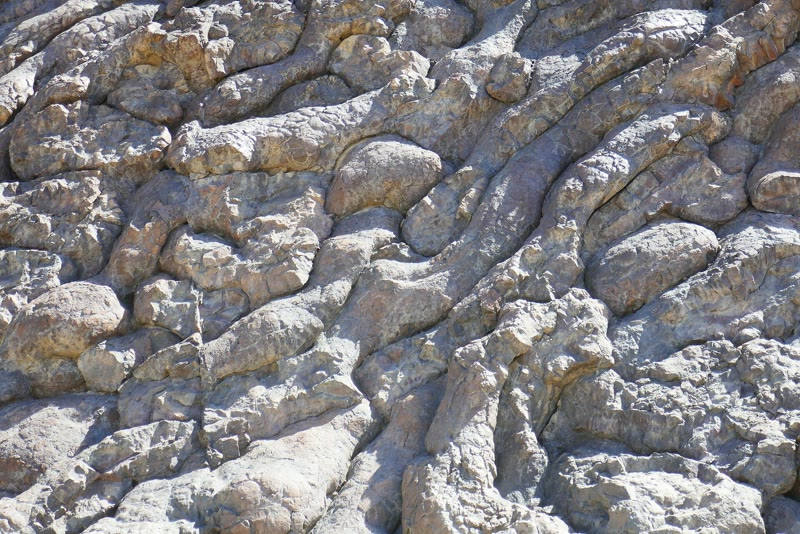
\includegraphics[width=0.6\linewidth]{images/book2/g12-duchoiselle-oman-pillows.jpg}

{\small Lava almohadillada de la \omterm{def:g12:mountain-building:ophiolite}{ofiolita} de Semail en Wadi Jizzi, Omán: lava
que se enfrió bajo el agua en forma de almohadillas redondeadas, hoy en tierra
firme. Fotografía de Lionel Duchoiselle (CC~BY-SA~3.0).}
\end{omfigure}
% ledger: photo:g12-oman-pillows

\section{Acortar la corteza}

Comprimido por los lados, un cuerpo de roca se rompe si está frío y es
frágil; si está lo bastante caliente para comportarse de forma plástica, se
pliega. Un cinturón montañoso está lleno de \omterm{def:g12:mountain-building:fold}{pliegues} y de fallas.
% ledger: earle:folds

\subsection{Pliegues}

\begin{definition}[Pliegue; anticlinal; sinclinal; eje del pliegue]\label{def:g12:mountain-building:fold}
Un \emph{pliegue}\index{pliegue} es una curvatura de las capas de roca. Sus
lados inclinados son los \emph{flancos}; se unen en la \emph{charnela}, donde
las capas están más curvadas, y la línea que recorre la charnela es el
\emph{eje del pliegue}\index{eje del pliegue}. Un \emph{anticlinal}\index{anticlinal} es un pliegue cuyas
capas se curvan hacia arriba, con los flancos inclinados alejándose del eje;
un \emph{sinclinal}\index{sinclinal} es un pliegue cuyas capas se curvan hacia
abajo, con los flancos inclinados hacia el eje.
\end{definition}
% ledger: earle:folds, tulane:fold-geometry

El plano que pasa por las charnelas de las capas sucesivas es el plano axial.
Los \omterm{def:g12:mountain-building:fold}{anticlinales} y los \omterm{def:g12:mountain-building:fold}{sinclinales} suelen ir por parejas: el flanco de uno es
el flanco del siguiente. Hay \omterm{def:g12:mountain-building:fold}{pliegues} de todos los tamaños, desde
microscópicos hasta de decenas de kilómetros. Una vez erosionado, un
\omterm{def:g12:mountain-building:fold}{anticlinal} muestra sus capas más antiguas en el núcleo, y un \omterm{def:g12:mountain-building:fold}{sinclinal} las más
jóvenes; un \omterm{def:g12:mountain-building:fold}{anticlinal} no es necesariamente una loma, ni un \omterm{def:g12:mountain-building:fold}{sinclinal} un
valle, porque la erosión sigue las capas duras y blandas más que la forma del
\omterm{def:g12:mountain-building:fold}{pliegue}.
% ledger: earle:folds, tulane:fold-geometry

\begin{omfigure}
\begin{tikzpicture}[x=1.2cm, y=1.2cm, font=\scriptsize]
  \def\W{6}\def\H{2.0}\def\dx{1.35}\def\dy{0.78}
  \tikzset{declare function={zb(\x,\c)=\c+0.8*cos(60*(\x-1.5));}}
  \colorlet{bandA}{omLithSchist!70}\colorlet{bandB}{omLithSand}\colorlet{bandC}{omLithShale}
  \colorlet{bandD}{icsJurassic!35}\colorlet{bandE}{icsTriassic!35}\colorlet{bandF}{icsCretaceous!45}
  % front face
  \begin{scope}
    \clip (0,0) rectangle (\W,\H);
    \fill[bandA] (0,0) rectangle (\W,\H);
    \foreach \c/\col in {0.0/bandB, 0.6/bandC, 1.2/bandD, 1.8/bandE, 2.4/bandF}
      \fill[\col] plot[domain=0:\W, samples=80, smooth] (\x,{zb(\x,\c)}) -- (\W,4) -- (0,4) -- cycle;
    \foreach \c in {0.0,0.6,1.2,1.8,2.4}
      \draw[black!55, line width=0.35pt] plot[domain=0:\W, samples=80, smooth] (\x,{zb(\x,\c)});
  \end{scope}
  % top face: outcrop bands (crossings of the top surface computed for these curves)
  \fill[bandE] (0,\H) -- (0.242,\H) -- ++(\dx,\dy) -- (\dx,\H+\dy) -- cycle;
  \fill[bandD] (0.242,\H) -- (2.758,\H) -- ++(\dx,\dy) -- (0.242+\dx,\H+\dy) -- cycle;
  \fill[bandE] (2.758,\H) -- (3.5,\H) -- ++(\dx,\dy) -- (2.758+\dx,\H+\dy) -- cycle;
  \fill[bandF] (3.5,\H) -- (5.5,\H) -- ++(\dx,\dy) -- (3.5+\dx,\H+\dy) -- cycle;
  \fill[bandE] (5.5,\H) -- (\W,\H) -- ++(\dx,\dy) -- (5.5+\dx,\H+\dy) -- cycle;
  \foreach \x in {0.242,2.758,3.5,5.5} \draw[black!55, line width=0.35pt] (\x,\H) -- ++(\dx,\dy);
  % right face: the layers meet it at constant heights (cylindrical folds)
  \foreach \lo/\hi/\col in {0.0/0.6/bandB, 0.6/1.2/bandC, 1.2/1.8/bandD, 1.8/2.0/bandE}
    \fill[\col] (\W,\lo) -- (\W+\dx,\lo+\dy) -- (\W+\dx,\hi+\dy) -- (\W,\hi) -- cycle;
  \foreach \y in {0.6,1.2,1.8} \draw[black!55, line width=0.35pt] (\W,\y) -- ++(\dx,\dy);
  % outline
  \draw[black, line width=0.5pt] (0,0) rectangle (\W,\H) (0,\H) -- (\dx,\H+\dy) -- (\W+\dx,\H+\dy) -- (\W,\H)
    (\W+\dx,\H+\dy) -- (\W+\dx,\dy) -- (\W,0);
  % fold axes on the top face, axial planes on the front face
  \draw[omThm, line width=1pt] (1.5,\H) -- ++(\dx,\dy);
  \draw[omDef, line width=1pt] (4.5,\H) -- ++(\dx,\dy);
  \draw[omThm, dashed, line width=0.6pt] (1.5,0) -- (1.5,\H);
  \draw[omDef, dashed, line width=0.6pt] (4.5,0) -- (4.5,\H);
  \node[anchor=south, omThm] at (1.5+\dx,\H+\dy) {anticlinal: eje del pliegue};
  \node[anchor=south, omDef] at (4.5+\dx,\H+\dy) {sinclinal: eje del pliegue};
  \draw[black!70] (3.2,0.95) -- (3.9,-0.35) node[anchor=north] {flanco};
  \draw[black!70] (1.5,1.4) circle (0.07) -- (0.4,-0.35) node[anchor=north] {charnela};
  \draw[black!70] (1.5,0.25) -- (2.0,-0.35) node[anchor=north] {plano axial};
\end{tikzpicture}

{\small Un \omterm{def:g12:mountain-building:fold}{anticlinal} y un \omterm{def:g12:mountain-building:fold}{sinclinal} cortados por una superficie de erosión
plana (bloque diagrama, sin escala). Los ejes de los \omterm{def:g12:mountain-building:fold}{pliegues} siguen las
charnelas; las líneas discontinuas son las trazas de los planos axiales. En la
superficie superior, el \omterm{def:g12:mountain-building:fold}{anticlinal} erosionado muestra capas más antiguas en su
núcleo, y el \omterm{def:g12:mountain-building:fold}{sinclinal}, más jóvenes.}
\end{omfigure}
% ledger: earle:folds, tulane:fold-geometry

\begin{omfigure}
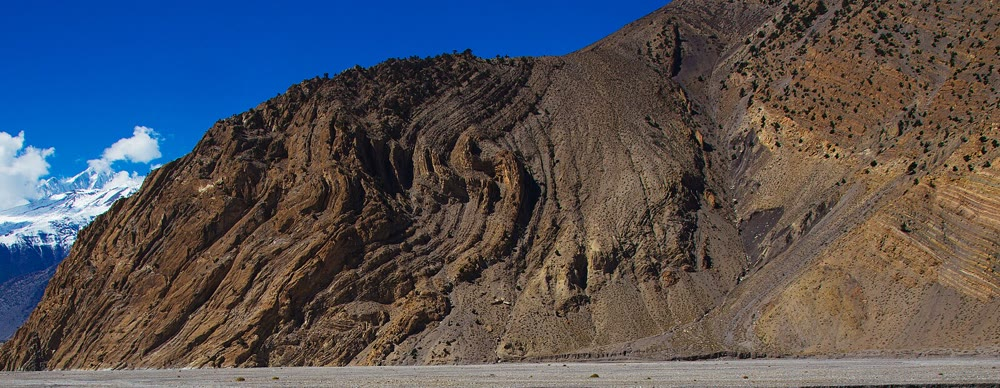
\includegraphics[width=0.95\linewidth]{images/book2/g12-hullot-kali-gandaki-folds.jpg}

{\small Capas de roca plegadas en un escarpe del Himalaya, a unos
\qty{3}{km} al noreste de Jomsom, en la garganta del Kali Gandaki, Nepal.
Fotografía de Jean-Marie Hullot (CC~BY~2.0).}
\end{omfigure}
% ledger: photo:g12-kali-gandaki

La cobertera de las Varden Hills está plegada del mismo modo, con mucha más
suavidad. Sus areniscas, calizas, lutitas y cretas se depositaron en
horizontal y después se curvaron en un \omterm{def:g12:mountain-building:fold}{anticlinal} y un \omterm{def:g12:mountain-building:fold}{sinclinal} cuyos flancos
buzan \ang{12}; una \omterm{def:g11:ocean-ridges:normal-fault}{falla normal} posterior los corta.
% ledger: region:name; model in figdata/shared/region.py (LIMB_DIP 12, AXIS_ANTI 3.5 km, AXIS_SYN 7.5 km)

\begin{omfigure}
\begin{tikzpicture}
\begin{axis}[omsection, x=1.25cm, y=0.003125cm, xmin=0, xmax=9.49, ymin=-700, ymax=650,
  xlabel={distancia desde A (\unit{km})}, ylabel={altitud (\unit{m})},
  ytick={-600,-300,0,300,600}, tick label style={font=\scriptsize}]
\addplot[fill=black!8, draw=black!50, line width=0.3pt, even odd rule] table {figdata/out/shared-region-section-unit-schist.dat};
\addplot[fill=icsTriassic!20, draw=black!50, line width=0.3pt, even odd rule] table {figdata/out/shared-region-section-unit-sandstone.dat};
\addplot[fill=icsJurassic!25, draw=black!50, line width=0.3pt, even odd rule] table {figdata/out/shared-region-section-unit-limestone.dat};
\addplot[fill=icsJurassic!8, draw=black!50, line width=0.3pt, even odd rule] table {figdata/out/shared-region-section-unit-shale.dat};
\addplot[fill=icsCretaceous!20, draw=black!50, line width=0.3pt, even odd rule] table {figdata/out/shared-region-section-unit-chalk.dat};
\addplot[fill=omLithAlluv, draw=black!50, line width=0.3pt, even odd rule] table {figdata/out/shared-region-section-unit-alluvium.dat};
\addplot[black, line width=0.7pt] table {figdata/out/shared-region-section-ground.dat};
\addplot[fault] table {figdata/out/shared-region-section-fault.dat};
% axis positions from figdata/grade-12/fold_shortening.py (section_anticline_km, section_syncline_km; the syncline lies on the hanging wall, shifted by the fault heave)
\draw[omThm, dashed, line width=0.7pt] (axis cs:3.162,-700) -- (axis cs:3.162,660);
\draw[omDef, dashed, line width=0.7pt] (axis cs:7.484,-700) -- (axis cs:7.484,660);
\node[anchor=south, omThm, font=\scriptsize] at (axis cs:3.162,660) {eje del anticlinal};
\node[anchor=south, omDef, font=\scriptsize] at (axis cs:7.484,660) {eje del sinclinal};
\node[anchor=south east, font=\small\bfseries] at (axis cs:0,650) {A};
\node[anchor=south west, font=\small\bfseries] at (axis cs:9.49,650) {B};
\node[font=\scriptsize, fill=white, inner sep=1pt] at (axis cs:1.2,-520) {esquisto};
\node[font=\scriptsize, fill=white, inner sep=1pt, anchor=east] at (axis cs:6.55,-450) {falla normal};
\end{axis}
\end{tikzpicture}

\smallskip
{\small\tikz\fill[black!8, draw=black!50] (0,0) rectangle (0.35,0.22);~esquisto \quad
\tikz\fill[icsTriassic!20, draw=black!50] (0,0) rectangle (0.35,0.22);~arenisca \quad
\tikz\fill[icsJurassic!25, draw=black!50] (0,0) rectangle (0.35,0.22);~caliza \quad
\tikz\fill[icsJurassic!8, draw=black!50] (0,0) rectangle (0.35,0.22);~lutita \quad
\tikz\fill[icsCretaceous!20, draw=black!50] (0,0) rectangle (0.35,0.22);~creta \quad
\omve{2.5}}

{\small Corte A--B a través de las Varden Hills, de suroeste a noreste. La
cobertera descansa sobre el zócalo de esquisto y está plegada en un \omterm{def:g12:mountain-building:fold}{anticlinal}
y un \omterm{def:g12:mountain-building:fold}{sinclinal}; la \omterm{def:g11:ocean-ridges:normal-fault}{falla normal}, más joven que los \omterm{def:g12:mountain-building:fold}{pliegues}, hunde el bloque
del noreste. La escala vertical está exagerada 2.5 veces, lo que hace que los
flancos parezcan más inclinados de lo que son. Datos: el modelo de la región
de la serie.}
\end{omfigure}
% ledger: region:name; computed in figdata/shared/region.py (section A-B)

\subsection{Fallas inversas, cabalgamientos y mantos de corrimiento}

Donde la corteza se comprime estando fría y frágil, se rompe a lo largo de
fallas de un tipo distinto de las \omterm{def:g11:ocean-ridges:normal-fault}{fallas normales} de la corteza estirada.

\begin{definition}[Falla inversa; cabalgamiento]\label{def:g12:mountain-building:thrust}
Una \emph{falla inversa}\index{falla inversa} es una falla inclinada a lo largo
de la cual el bloque situado por encima del plano de falla ha subido respecto
al bloque de debajo. Las fallas inversas se forman donde la corteza se
comprime. Un \emph{cabalgamiento}\index{cabalgamiento} es una falla inversa de
buzamiento suave, de menos de \ang{45}.
\end{definition}
% ledger: earle:reverse-thrust, tulane:fold-geometry

Un \omterm{def:g12:mountain-building:thrust}{cabalgamiento} puede transportar una lámina de roca a lo largo de decenas de
kilómetros, y entonces unas rocas más antiguas quedan encima de otras más
jóvenes, al revés del orden en que se depositaron. En las Montañas Rocosas, el
\omterm{def:g12:mountain-building:thrust}{cabalgamiento} de McConnell ha empujado un apilamiento de rocas sedimentarias de
unos \qty{800}{m} de espesor unos \qty{40}{km} de oeste a este: una caliza de
unos 500 millones de años descansa hoy sobre una fangolita de unos 75 millones
de años.
% ledger: earle:reverse-thrust

\begin{definition}[Manto de corrimiento]\label{def:g12:mountain-building:nappe}
Un \emph{manto de corrimiento}\index{manto de corrimiento} es una gran lámina
de roca que ha sido transportada una larga distancia, a menudo decenas de
kilómetros, sobre las rocas de debajo, a lo largo de un \omterm{def:g12:mountain-building:thrust}{cabalgamiento} casi
horizontal.
\end{definition}
% ledger: ngu:nappe, earle:reverse-thrust

Un \omterm{def:g12:mountain-building:nappe}{manto de corrimiento} puede transportar rocas formadas muy lejos, incluso
láminas de fondo oceánico; él mismo puede estar plegado, con sus capas
invertidas. Los cinturones montañosos apilan \omterm{def:g12:mountain-building:nappe}{mantos de corrimiento} unos sobre
otros. Más tarde, la erosión abre huecos en un manto, que forman ventanas
hacia las rocas de debajo, y deja fragmentos aislados de él sobre las rocas
más jóvenes.
% ledger: ngu:nappe

\begin{omfigure}
\begin{tikzpicture}[x=1.0cm, y=1.0cm, font=\scriptsize]
  % rocks in place (younger), flat-lying
  \fill[icsCretaceous!25] (0,-1.6) rectangle (12,-0.4);
  \fill[icsJurassic!25] (0,-1.6) rectangle (12,-1.1);
  \draw[black!50, line width=0.3pt] (0,-1.1) -- (12,-1.1);
  \fill[white] (5.6,-0.4) -- (6.2,-0.62) -- (6.8,-0.4) -- cycle;
  % the nappe (older rocks) above a nearly flat thrust, cut by erosion
  \fill[omLithSchist!80] (0.8,-0.4) .. controls (1.2,0.35) and (1.9,0.35) .. (2.3,-0.4) -- cycle;
  \fill[omLithSchist!80] (3.2,-0.4) .. controls (3.9,0.9) and (4.8,0.9) .. (5.6,-0.4) -- cycle;
  \fill[omLithSchist!80] (6.8,-0.4) .. controls (7.1,0.9) and (7.7,1.3) .. (8.4,1.25) -- (12,0.9) -- (12,-0.4) -- cycle;
  % ground surface
  \draw[black, line width=0.6pt] (0,-0.4) -- (0.8,-0.4) .. controls (1.2,0.35) and (1.9,0.35) .. (2.3,-0.4)
     -- (3.2,-0.4) .. controls (3.9,0.9) and (4.8,0.9) .. (5.6,-0.4) -- (6.2,-0.62) -- (6.8,-0.4)
     .. controls (7.1,0.9) and (7.7,1.3) .. (8.4,1.25) -- (12,0.9);
  % thrust traces (teeth on the block that moved over)
  \draw[thrust fault] (0.8,-0.4) -- (2.3,-0.4);
  \draw[thrust fault] (3.2,-0.4) -- (5.6,-0.4);
  \draw[thrust fault] (6.8,-0.4) -- (12,-0.4);
  \draw[-{Stealth[length=2mm]}, line width=0.9pt] (11.4,1.45) -- (9.6,1.6);
  \node[anchor=south] at (10.5,1.55) {movimiento del manto};
  \node at (9.9,0.3) {manto: rocas más antiguas};
  \node[fill=white, inner sep=1pt] at (2.0,-0.85) {rocas en su sitio: más jóvenes};
  \draw[black!60] (1.55,0.0) -- (1.3,0.8) node[anchor=south] {fragmento aislado};
  \draw[black!60] (6.2,-0.58) -- (6.2,-0.68) node[anchor=north, fill=white, inner sep=1pt] {ventana};
  \draw[black!60] (9.0,-0.42) -- (9.3,-0.68) node[anchor=north, fill=white, inner sep=1pt] {cabalgamiento};
\end{tikzpicture}

{\small Un \omterm{def:g12:mountain-building:nappe}{manto de corrimiento} (sin escala): una lámina de rocas más antiguas
transportada a lo largo de un \omterm{def:g12:mountain-building:thrust}{cabalgamiento} casi horizontal sobre rocas más
jóvenes que han permanecido en su sitio. La erosión ha abierto en él una
ventana y ha dejado un fragmento aislado a la izquierda. Los dientes del
\omterm{def:g12:mountain-building:thrust}{cabalgamiento} apuntan hacia el bloque que se ha desplazado por encima.}
\end{omfigure}
% ledger: ngu:nappe, earle:reverse-thrust

\begin{omfigure}
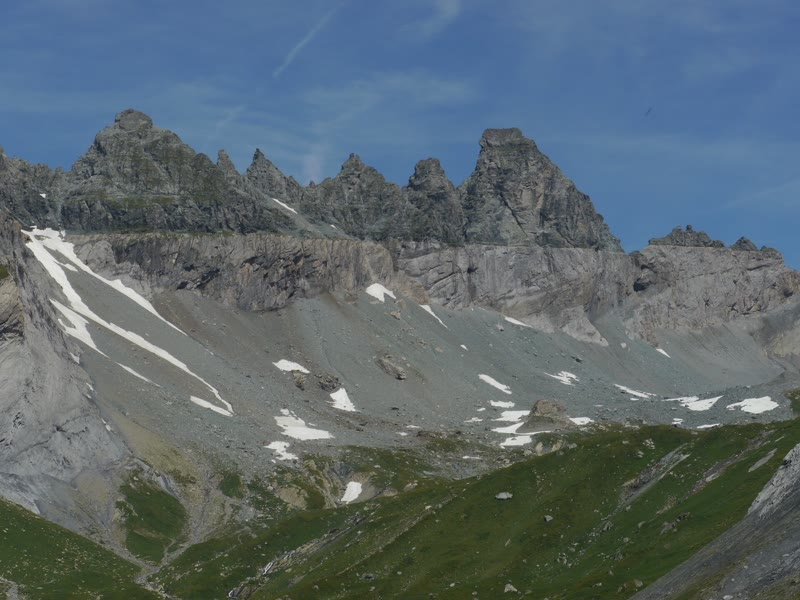
\includegraphics[width=0.5\linewidth]{images/book2/g12-heine-glarus-thrust.jpg}

{\small El \omterm{def:g12:mountain-building:thrust}{cabalgamiento} de Glarus, en los Alpes del este de Suiza. Las rocas
oscuras de las cumbres, depositadas en el Pérmico, hace entre unos 299 y 252
millones de años, descansan sobre rocas más claras y mucho más jóvenes; el
\omterm{def:g12:mountain-building:thrust}{cabalgamiento} es el límite nítido entre ellas. Las rocas superiores se han
desplazado de 40 a \qty{50}{km}. Fotografía de Christian Heine (CC~BY-SA~3.0).}
\end{omfigure}
% ledger: photo:g12-glarus (Verrucano, Permian; displacement 40-50 km, Pfiffner 1985), ics:base.Permian, ics:base.Triassic

\subsection{Medir el acortamiento}

Los \omterm{def:g12:mountain-building:fold}{pliegues} y los \omterm{def:g12:mountain-building:thrust}{cabalgamientos} acortan la corteza en la dirección en que
se comprime.

\begin{definition}[Acortamiento]\label{def:g12:mountain-building:shortening}
El \emph{acortamiento}\index{acortamiento} de una capa es la fracción de su
longitud que ha perdido: si medía $L_0$ y ahora abarca $L$,
\[
  e = \frac{L_0 - L}{L_0}.
\]
\end{definition}

Para medirlo hace falta la longitud original $L_0$. En muchos \omterm{def:g12:mountain-building:fold}{pliegues} las
capas conservan su espesor al curvarse, deslizándose unas sobre otras como las
páginas de un libro doblado; una capa así no se estira a lo largo de su
longitud. Eso da la longitud original.
% ledger: tulane:fold-geometry (flexural folds keep their thickness)

\begin{proposition}[El acortamiento de una capa plegada]\label{prop:g12:mountain-building:shortening}
Si una capa se ha plegado sin estirarse ni comprimirse a lo largo de sí misma,
su longitud original $L_0$ es su longitud medida a lo largo de la capa
plegada. Para un \omterm{def:g12:mountain-building:fold}{pliegue} de flancos rectos que buzan un ángulo $\theta$,
\[
  e = 1 - \cos\theta .
\]
\end{proposition}

\begin{proof}
Al desplegar la capa, sin estirarla, queda extendida en horizontal con su
longitud intacta; así que $L_0$ es la longitud a lo largo de la capa. En un
flanco recto de longitud $\ell$ que buza $\theta$, la distancia horizontal
recorrida es $\ell\cos\theta$ (triángulo rectángulo). Sumando todos los
flancos, la capa de longitud $L_0$ abarca $L = L_0\cos\theta$, y $e = (L_0 - L_0\cos\theta)/L_0 =
1 - \cos\theta$.
\end{proof}

\begin{omfigure}
\begin{tikzpicture}
\begin{axis}[name=sine, x=2.0cm, y=2.0cm, axis lines=none,
  xmin=-0.05, xmax=2.25, ymin=-0.4, ymax=0.8, clip=false]
% computed in figdata/grade-12/fold_shortening.py (part sine: A/lambda = 0.25, e = 31.7 %)
\addplot[omLithSand!80!black, line width=1.6pt] table[x=x, y=y] {figdata/out/grade-12-fold_shortening-sine.dat};
\draw[omThm, line width=1.6pt] (axis cs:0,0.62) -- (axis cs:2.196,0.62);
\draw[black!60, |-|] (axis cs:0,-0.32) -- node[below, font=\scriptsize] {$L$ (hoy)} (axis cs:1.5,-0.32);
\node[anchor=south west, font=\scriptsize, omThm] at (axis cs:0,0.64) {$L_0$: la misma capa desplegada};
\end{axis}
\begin{axis}[omrecord, at={(sine.east)}, anchor=west, xshift=1.4cm, width=0.46\linewidth, height=4.6cm,
  xmin=0, xmax=80, ymin=0, ymax=85, xlabel={buzamiento de los flancos $\theta$ (\unit{\degree})},
  ylabel={acortamiento $e$ (\unit{\percent})}, xtick={0,20,...,80}]
% computed in figdata/grade-12/fold_shortening.py (part dip: e = 1 - cos theta)
\addplot[omProp, line width=1pt] table[x=theta, y=e_pct] {figdata/out/grade-12-fold_shortening-dip.dat};
\addplot[only marks, mark=*, mark size=1.6pt, omThm] coordinates {(12,2.185) (30,13.397) (60,50)};
\node[anchor=south, font=\scriptsize, align=center] at (axis cs:12,6) {Varden:\\\qty{2.2}{\percent}};
\node[anchor=west, font=\scriptsize] at (axis cs:32,10) {\qty{13}{\percent}};
\node[anchor=south east, font=\scriptsize] at (axis cs:60,51) {\qty{50}{\percent}};
\end{axis}
\end{tikzpicture}

{\small A la izquierda: una capa plegada abarca $L$; extendida en horizontal,
sin estirarla, mide $L_0$ (aquí los \omterm{def:g12:mountain-building:fold}{pliegues} tienen una altura de un cuarto de
su longitud de onda, y $L$ es el \qty{68}{\percent} de $L_0$). A la derecha:
el \omterm{def:g12:mountain-building:shortening}{acortamiento} de un \omterm{def:g12:mountain-building:fold}{pliegue} de flancos rectos, $1 - \cos\theta$, frente al
buzamiento de sus flancos. Los \omterm{def:g12:mountain-building:fold}{pliegues} suaves acortan muy poco una capa.}
\end{omfigure}
% values: sine_025_e_pct 31.68 (L/L0 = 0.683); varden_e_pct 2.1852; chevron_30 13.397; chevron_60 50 (fold_shortening.py)

\begin{method}[Medir el acortamiento en un corte geológico]\label{met:g12:mountain-building:shortening}
\begin{enumerate}
  \item Comprueba que el corte está dibujado a escala real. Si su escala
        vertical está exagerada, los buzamientos y las longitudes a lo largo de
        las capas salen demasiado grandes: vuelve a dibujarlo, o corrige
        primero cada buzamiento.
  \item Elige un límite entre capas que pueda seguirse a través de todo el
        corte; donde lo corte una falla, une los dos extremos cortados como
        estaban antes de que la falla se moviera.
  \item Mide su longitud a lo largo de la capa, $L_0$: síguelo con un hilo,
        o suma tramos rectos cortos.
  \item Mide la distancia horizontal entre sus dos extremos, $L$.
  \item Calcula $e = (L_0 - L)/L_0$; para flancos rectos de buzamiento
        conocido, $e = 1 - \cos\theta$ lo da directamente.
\end{enumerate}
\end{method}

\begin{example}[Los pliegues de Varden]\label{ex:g12:mountain-building:varden}
Los flancos de los \omterm{def:g12:mountain-building:fold}{pliegues} de Varden buzan \ang{12}, así que la cobertera se
acortó en $e = 1 - \cos\ang{12} = 1 - 0.978 = 0.022$, alrededor del
\qty{2.2}{\percent}: una franja de la región que hoy mide \qty{10}{km} de
ancho medía $10/\cos\ang{12} \approx
\qty{10.22}{km}$ antes del plegamiento. Medidos sobre el corte A--B tal como
está dibujado, los flancos parecerían buzar unos \ang{28}, porque la escala
vertical está exagerada 2.5 veces: $\tan\theta$ queda multiplicada por 2.5, y $\arctan(2.5
\tan\ang{12}) \approx \ang{28}$. Tomado al pie de la letra, eso daría un
\omterm{def:g12:mountain-building:shortening}{acortamiento} del \qty{12}{\percent}, más de cinco veces demasiado.
\end{example}
% values: varden_e_pct 2.1852, varden_L0_for_10km 10.223 (fold_shortening.py); arctan(2.5 x 0.2126) = 27.98 deg; 1 - cos 27.98 = 0.117

Los \omterm{def:g12:mountain-building:fold}{pliegues} suaves absorben poco. Un cinturón muy plegado, con flancos que
buzan \ang{60}, se ha acortado a la mitad; y un solo \omterm{def:g12:mountain-building:thrust}{cabalgamiento} casi
horizontal que ha transportado un \omterm{def:g12:mountain-building:nappe}{manto de corrimiento} \qty{40}{km} absorbe
\qty{40}{km} de \omterm{def:g12:mountain-building:shortening}{acortamiento}, tanto como un cinturón muy ancho de \omterm{def:g12:mountain-building:fold}{pliegues}
suaves.

\section{Engrosamiento y levantamiento}

El \omterm{def:g12:mountain-building:shortening}{acortamiento} no destruye la roca. Una franja de corteza comprimida hasta
una fracción de su anchura anterior conserva su volumen, así que debe
engrosarse: si una corteza de espesor
$H_0$ se acorta de una anchura $L_0$ a $L$ a lo largo de todo el cinturón,
su sección conserva su área, $H L = H_0 L_0$, y
\[
  H = H_0\,\frac{L_0}{L} = \frac{H_0}{1 - e}.
\]
Una corteza de \qty{35}{km} de espesor acortada un \qty{50}{\percent} pasa a
tener \qty{70}{km} de espesor. Luego la \omterm{def:g11:lithosphere-asthenosphere:isostasy}{isostasia} hace el resto: una corteza
más gruesa flota más alta, sobre una \omterm{def:g12:continental-crust:root}{raíz} más profunda (la
\cref{prop:g11:lithosphere-asthenosphere:airy}). Con el modelo de Airy y las
densidades del recordatorio, una corteza más gruesa en
$\Delta H$ se eleva $\Delta H\,(\rho_m - \rho_c)/\rho_m = \Delta H
\times 550/3380$ más, alrededor de un sexto del espesor añadido; los otros
cinco sextos forman la \omterm{def:g12:continental-crust:root}{raíz}. La corteza tiene de \num{35} a \qty{40}{km} de
espesor lejos de los cinturones montañosos, y de 50 a \qty{70}{km} bajo
ellos: cuanto más altas son las montañas, más gruesa es la corteza.
% ledger: tulane:roots, cm95:crust, data:prem

Así llegó la caliza de un fondo marino a la cima del Everest: depositada en el
fondo de un mar, fue transportada hacia el norte con la India, apilada en las
láminas cabalgantes del Himalaya y elevada a medida que la corteza de debajo
se engrosaba y subía. Ese movimiento vertical de la corteza se llama
levantamiento.
% ledger: sakai05:summit, sakai05:stacking, tulane:roots (uplift), usgs:himalaya-collision

\section{Dos cordilleras}

\subsection{El Himalaya}

El Himalaya se extiende \qty{2900}{km} a lo largo de la frontera entre la
India y el Tíbet. Hace unos 80 millones de años, la India estaba unos
\qty{6400}{km} al sur de Asia, al otro lado de un océano, y avanzaba hacia el
norte a unos \qty{9}{cm} al año; se encontró con Asia hace entre 40 y 50
millones de años, y su avance hacia el norte se frenó entonces. Las
reconstrucciones de placas muestran el viaje con detalle: construidas a partir
de muchos tipos de pruebas, entre ellas las trazas de los puntos calientes
(el \cref{ch:g11:plate-motions}), hacen retroceder las placas en el tiempo paso
a paso.
% ledger: usgs:himalaya-collision, muller19:frame, muller22:frame

\begin{omfigure}
\begin{tikzpicture}
\begin{axis}[omrecord, omage, name=lat, width=0.5\linewidth, height=5.2cm,
  xmin=0, xmax=100, ymin=-45, ymax=35, xlabel={edad (\unit{Ma})}, ylabel={latitud (\unit{\degree})},
  xtick={0,20,...,100}, ytick={-40,-20,...,40},
  legend style={font=\scriptsize, at={(0.98,0.03)}, anchor=south east, fill=white}]
% computed in figdata/grade-12/india_drift.py (part lat; GPlates Web Service, MULLER2022 and MULLER2019)
\fill[omThm!12] (axis cs:40,-45) rectangle (axis cs:50,35);
\addplot[omThm, line width=1.1pt] table[x=age, y=m22_india] {figdata/out/grade-12-india_drift-lat.dat};
\addplot[omThm, dashed, line width=0.8pt] table[x=age, y=m19_india] {figdata/out/grade-12-india_drift-lat.dat};
\addplot[omDef, line width=1.1pt] table[x=age, y=m22_lhasa] {figdata/out/grade-12-india_drift-lat.dat};
\addplot[black!50, line width=0.4pt, forget plot] coordinates {(0,0) (100,0)};
\legend{{centro de la India (2022)}, {centro de la India (2019)}, {Lhasa (2022)}}
\end{axis}
\begin{axis}[omrecord, omage, at={(lat.east)}, anchor=west, xshift=1.9cm, width=0.42\linewidth, height=5.2cm,
  xmin=0, xmax=100, ymin=0, ymax=160, xlabel={edad (\unit{Ma})},
  ylabel={velocidad hacia el norte (\unit{mm/yr})}, xtick={0,20,...,100}]
% computed in figdata/grade-12/india_drift.py (part steps: 5-Myr steps)
\fill[omThm!12] (axis cs:40,0) rectangle (axis cs:50,160);
\addplot[omThm, line width=1pt] table[x=age, y=m22] {figdata/out/grade-12-india_drift-steps.dat};
\addplot[omThm, dashed, line width=0.7pt] table[x=age, y=m19] {figdata/out/grade-12-india_drift-steps.dat};
\end{axis}
\end{tikzpicture}

{\small A la izquierda: la latitud de un punto del centro de la India
(\ang{78}~E, \ang{20}~N hoy) y de Lhasa, al norte de la \omterm{def:g12:mountain-building:suture}{sutura}, durante los
últimos 100 millones de años, en dos reconstrucciones de placas publicadas
(2022 y 2019). A la derecha: la velocidad de la India hacia el norte en cada
paso de 5 millones de años. La banda sombreada marca el intervalo de hace 40 a
50 millones de años. Datos: R.~D.~Müller y colaboradores (2019, 2022),
calculado con el GPlates Web Service.}
\end{omfigure}
% ledger: data:b2-gws-india, muller22:frame, muller19:frame; values: speed_65_50 128.5, speed_40_0 40.06, fastest 145.8 (50-55 Ma) (india_drift.py)

Las dos reconstrucciones coinciden con un margen de pocos grados. Entre hace
65 y 50 millones de años, la India avanzaba hacia el norte a unos
\qty{13}{cm} al año; entre hace 50 y 40 millones de años su velocidad cayó, y
desde hace 40 millones de años avanza a unos \qty{4}{cm} al año, menos de un
tercio. Lhasa, en el lado asiático, también se desplazó hacia el norte, pero
mucho más despacio.
% values: speed_65_50 128.5 mm/yr, speed_40_0 40.06 mm/yr, slowdown_ratio 0.312 (india_drift.py)

\begin{example}[La velocidad de la India]\label{ex:g12:mountain-building:india}
En la reconstrucción de 2022, el centro de la India estaba a \ang{12.10}~S
hace 60 millones de años y a \ang{0.68}~S hace 50 millones de años. Un grado
de latitud mide
$2\pi R/360 = 2\pi \times \qty{6371}{km}/360 \approx \qty{111.2}{km}$. La
India avanzó hacia el norte $(12.10 - 0.68) \times 111.2 \approx \qty{1270}{km}$ en 10 millones de años: \qty{127}{km} por millón de años, es
decir, $\qty{127e6}{mm} /
\num{e6}\text{ años} = \qty{127}{mm}$, unos \qty{13}{cm}, al año.
\end{example}
% ledger: data:b2-gws-india, earth:Rmean; values: lat 60 Ma -12.0964, 50 Ma -0.6801 (india_drift-lat)

La desaceleración se interpreta como la huella de la colisión: la \omterm{def:g12:continental-crust:continental-crust}{corteza
continental} que llegaba a la fosa no podía hundirse, y la India quedó
frenada. La fecha exacta del primer contacto sigue en debate: las
estimaciones van de hace unos 60 a 54 millones de años, y algunos geólogos
sostienen que la India chocó primero con una cadena de islas volcánicas y
solo alcanzó la propia Asia hace unos 34 millones de años. La India no se ha
detenido: los polos de rotación de las placas actuales la acercan a Eurasia a
unos \qty{4.5}{cm} al año a través del Himalaya (el
\cref{ch:g11:plate-motions}), y el empuje desplaza partes de Asia hacia el
este.
% ledger: usgs:himalaya-collision, najman21:collision-age; values: today_in_eu_speed 44.99 mm/yr (india_drift.py, from nnr56:poles)

Al norte del Himalaya, la meseta del Tíbet tiene unos \qty{4600}{m} de altura
media, sobre una corteza de unos \qty{70}{km} de espesor
(el \cref{ch:g11:lithosphere-asthenosphere}). Entre la India y el Tíbet se
encuentra la \omterm{def:g12:mountain-building:suture}{sutura} del Indo--Tsangpo con sus \omterm{def:g12:mountain-building:ophiolite}{ofiolitas}; al sur de ella, el
Himalaya está formado en gran parte por sedimentos depositados en el borde
norte de la India, después apilados, plegados y fallados, entre ellos la
caliza de la cumbre del Everest.
% ledger: karplus:tibet-moho, liu20:itsz, sakai05:stacking, sakai05:summit; Book 1: usgs:himalaya (Tibetan Plateau about 4600 m)

\subsection{Los Alpes y todo un cinturón}

Los Alpes tienen una historia parecida a menor escala: se levantaron donde
África chocó con Europa. También contienen \omterm{def:g12:mountain-building:ophiolite}{ofiolitas} y grandes
\omterm{def:g12:mountain-building:thrust}{cabalgamientos}: en el \omterm{def:g12:mountain-building:thrust}{cabalgamiento} de Glarus, rocas pérmicas han sido
transportadas sobre otras mucho más jóvenes. Los Alpes y el Himalaya
pertenecen a un mismo y largo cinturón de montañas, que pasa por los Zagros de
Irán, donde África y la India han chocado con Eurasia.
% ledger: earle:collision, photo:g12-glarus

\begin{omfigure}
\begin{tikzpicture}
\begin{axis}[axis equal image, xmin=-12, xmax=105, ymin=18, ymax=52, width=\linewidth,
  tick label style={font=\scriptsize}, xtick={0,30,60,90}, ytick={20,30,40,50},
  xticklabel={$\pgfmathprintnumber{\tick}^\circ$}, yticklabel={$\pgfmathprintnumber{\tick}^\circ$},
  axis background/.style={fill=omSea}, legend columns=3,
  legend style={font=\scriptsize, at={(0.5,-0.12)}, anchor=north, /tikz/every even column/.append style={column sep=5pt}}]
\addplot[fill=omLithAlluv, draw=black!45, line width=0.2pt, forget plot] table {figdata/out/shared-geo-land.dat};
% computed in figdata/grade-12/alpine_belt.py; ledger: data:etopo1, data:usgs-comcat
\addplot[only marks, mark=square*, mark size=1.15pt, omLithSand!85!black] table[x=lon, y=lat] {figdata/out/grade-12-alpine_belt-high.dat};
\addplot[only marks, mark=square*, mark size=1.15pt, omThm!75!black] table[x=lon, y=lat] {figdata/out/grade-12-alpine_belt-higher.dat};
\addplot[only marks, mark=*, mark size=0.7pt, black] table[x=lon, y=lat] {figdata/out/grade-12-alpine_belt-quakes.dat};
\addplot[omDef, line width=0.9pt, forget plot] table {figdata/out/shared-geo-school-collision.dat};
\addplot[black!70, line width=0.5pt, forget plot] table {figdata/out/shared-geo-school-subduction.dat};
\legend{{más de \qty{1500}{m}}, {más de \qty{3500}{m}}, {terremoto de magnitud 6 o más}}
\coordinate (alps) at (axis cs:9,48);
\coordinate (zagros) at (axis cs:46,23.5);
\coordinate (zagrosbelt) at (axis cs:50.5,31.5);
\coordinate (himal) at (axis cs:84,24);
\coordinate (tibet) at (axis cs:88,33);
\coordinate (arrA) at (axis cs:77,19.5);
\coordinate (arrB) at (axis cs:79.2,25);
\end{axis}
% labels drawn after the axis, so that no earthquake dot covers them
\node[font=\scriptsize, fill=white, inner sep=1pt, anchor=south] at (alps) {Alpes};
\draw[black!60, line width=0.4pt] (zagros) -- (zagrosbelt);
\node[font=\scriptsize, fill=white, inner sep=1pt] at (zagros) {Zagros};
\node[font=\scriptsize, fill=white, inner sep=1pt, anchor=west] at (himal) {Himalaya};
\node[font=\scriptsize, fill=white, inner sep=1pt] at (tibet) {meseta del Tíbet};
\draw[-{Stealth[length=2mm]}, line width=1pt, omProp] (arrA) -- (arrB);
\end{tikzpicture}

{\small El cinturón de montañas jóvenes del Atlántico al Tíbet: relieve alto
(cada cuadrado es una celda de 1 grado), terremotos superficiales de magnitud
6 o más de 1976 a 2025 (a menos de \qty{70}{km} de profundidad) y los límites
de colisión entre placas (línea azul). La flecha muestra el movimiento de la
India hacia Eurasia. Datos: ETOPO1, catálogo de terremotos del USGS, límites
de placas de Bird (2003), tierras de Natural Earth.}
\end{omfigure}
% ledger: data:etopo1, data:usgs-comcat, data:pb2002, data:ne-land; values: n_quakes 398 (alpine_belt.py)

El relieve alto y los terremotos siguen la misma banda estrecha. La colisión
no ha terminado: los terremotos muestran que la corteza sigue rompiéndose a lo
largo de todo el cinturón, y que las montañas siguen formándose.

\section{Ejercicios}

\begin{exercise}[$\star$]\label{exo:g12:mountain-building:1}
Asocia cada término con su descripción: \omterm{def:g12:mountain-building:fold}{anticlinal}, \omterm{def:g12:mountain-building:fold}{sinclinal},
\omterm{def:g12:mountain-building:thrust}{cabalgamiento}, \omterm{def:g12:mountain-building:nappe}{manto de corrimiento}, \omterm{def:g12:mountain-building:suture}{sutura}, \omterm{def:g12:mountain-building:ophiolite}{ofiolita}. (a) una \omterm{def:g12:mountain-building:thrust}{falla inversa}
de buzamiento suave; (b) un fragmento de fondo oceánico hallado en tierra
firme; (c) un \omterm{def:g12:mountain-building:fold}{pliegue} cuyos flancos buzan hacia su eje; (d) la línea por la
que se unieron dos continentes; (e) un \omterm{def:g12:mountain-building:fold}{pliegue} cuyos flancos buzan alejándose
de su eje; (f) una gran lámina de roca transportada lejos a lo largo de un
\omterm{def:g12:mountain-building:thrust}{cabalgamiento}.
\end{exercise}

\begin{exercise}[$\star$]\label{exo:g12:mountain-building:2}
A un lado y otro de un valle, las capas del lado oeste buzan \ang{20} hacia
el oeste y las del lado este buzan \ang{20} hacia el este. (1) ¿El \omterm{def:g12:mountain-building:fold}{pliegue}
que hay entre ellas es un \omterm{def:g12:mountain-building:fold}{anticlinal} o un \omterm{def:g12:mountain-building:fold}{sinclinal}? (2) Tras la erosión, ¿se
encuentran a lo largo de su eje las capas más antiguas o las más jóvenes?
(3) ¿Tiene que estar el valle sobre un \omterm{def:g12:mountain-building:fold}{sinclinal}?
\end{exercise}

\begin{exercise}[$\star$]\label{exo:g12:mountain-building:3}
Una capa está plegada con flancos rectos que buzan \ang{30}. (1) Calcula su
\omterm{def:g12:mountain-building:shortening}{acortamiento}. (2) Hoy abarca \qty{6.0}{km}. ¿Cuánto medía?
\end{exercise}

\begin{exercise}[$\star$]\label{exo:g12:mountain-building:4}
(1) A lo largo de una falla, el bloque situado por encima del plano de falla
ha bajado. ¿Es una \omterm{def:g11:ocean-ridges:normal-fault}{falla normal} o inversa, y la corteza se estiró o se
comprimió? (2) Una \omterm{def:g12:mountain-building:thrust}{falla inversa} buza \ang{25}: ¿es un \omterm{def:g12:mountain-building:thrust}{cabalgamiento}?
\end{exercise}

\begin{exercise}[$\star$]\label{exo:g12:mountain-building:5}
(1) Ordena de arriba abajo estas rocas de una \omterm{def:g12:mountain-building:ophiolite}{ofiolita}: \omterm{def:g11:ocean-ridges:gabbro}{gabro}, sedimentos
marinos, \omterm{def:g11:ocean-ridges:peridotite}{peridotita}, basaltos almohadillados, complejo de \omterm{def:g11:igneous-rocks:intrusion}{diques} laminares.
(2) ¿Por qué los basaltos almohadillados muestran que la roca se formó bajo el
agua? (3) ¿Por qué se encuentran \omterm{def:g12:mountain-building:ophiolite}{ofiolitas} a lo largo de las \omterm{def:g12:mountain-building:suture}{suturas}?
\end{exercise}

\begin{exercise}[$\star\star$]\label{exo:g12:mountain-building:6}
En un corte geológico a escala real, se sigue un límite de arenisca a lo
largo de cuatro tramos rectos de \qty{2.1}{km}, \qty{1.8}{km}, \qty{2.4}{km}
y \qty{1.6}{km}; sus extremos están a \qty{6.0}{km} uno de otro. (1) Calcula
el \omterm{def:g12:mountain-building:shortening}{acortamiento}. (2) Si los cuatro flancos buzan todos el mismo ángulo,
¿cuál es?
\end{exercise}

\begin{exercise}[$\star\star$]\label{exo:g12:mountain-building:7}
El bloque superior de un \omterm{def:g12:mountain-building:thrust}{cabalgamiento} que buza \ang{10} se ha desplazado
\qty{45}{km} a lo largo del plano de falla. (1) ¿Cuánto se ha desplazado en
horizontal? (2) ¿Cuánto ha subido? (3) ¿Qué anchura debería tener un cinturón
de \omterm{def:g12:mountain-building:fold}{pliegues} con flancos que buzan \ang{12} para absorber el mismo
\omterm{def:g12:mountain-building:shortening}{acortamiento} horizontal?
\end{exercise}

\begin{exercise}[$\star\star$]\label{exo:g12:mountain-building:8}
A lo largo del \omterm{def:g12:mountain-building:thrust}{cabalgamiento} de McConnell, una caliza de unos 500 millones de
años descansa sobre una fangolita de unos 75 millones de años. (1) ¿Qué
principio de la datación relativa engañaría a un geólogo que ignorara la
falla? (2) ¿Cuánto más antigua es la roca superior? (3) La lámina cabalgante
tiene unos \qty{800}{m} de espesor y se desplazó \qty{40}{km}: ¿cuántas veces
su propio espesor es eso?
\end{exercise}

\begin{exercise}[$\star\star$]\label{exo:g12:mountain-building:9}
En la reconstrucción de 2022, el centro de la India estaba a \ang{30.23}~S
hace 80 millones de años y a \ang{19.38}~S hace 66 millones de años. (1) ¿Cuánto
avanzó hacia el norte? (2) ¿A qué velocidad media, en \unit{cm} al año?
(3) Compáralo con el resumen del Servicio Geológico de los Estados Unidos,
unos \qty{9}{m} por siglo.
\end{exercise}

\begin{exercise}[$\star\star$]\label{exo:g12:mountain-building:10}
Una corteza de \qty{35}{km} de espesor se acorta un \qty{40}{\percent} en
todo un cinturón. (1) ¿Qué espesor alcanza? (2) Con $\rho_c =
\qty{2830}{kg/m^3}$ y $\rho_m = \qty{3380}{kg/m^3}$, ¿cuánto más alta se
eleva, y qué profundidad tiene su \omterm{def:g12:continental-crust:root}{raíz} añadida?
\end{exercise}

\begin{exercise}[$\star\star$]\label{exo:g12:mountain-building:11}
En un corte dibujado con la escala vertical exagerada 3 veces, un flanco
parece buzar \ang{40}. (1) ¿Cuál es su buzamiento real? (2) Calcula el
\omterm{def:g12:mountain-building:shortening}{acortamiento} a partir del buzamiento real y del buzamiento leído en el
dibujo. (3) ¿Por qué los cortes que se usan para medir el \omterm{def:g12:mountain-building:shortening}{acortamiento} deben
dibujarse a escala real?
\end{exercise}

\begin{exercise}[$\star\star\star$]\label{exo:g12:mountain-building:12}
Los \omterm{def:g12:mountain-building:fold}{pliegues} redondeados dibujados en este capítulo, con una altura de un
cuarto de su longitud de onda, tienen un \omterm{def:g12:mountain-building:shortening}{acortamiento} del
\qty{31.7}{\percent}; su buzamiento máximo es de unos \ang{57.5}. (1) Una
capa plegada así abarca \qty{10}{km}: ¿cuánto medía? (2) Calcula el
\omterm{def:g12:mountain-building:shortening}{acortamiento} de un \omterm{def:g12:mountain-building:fold}{pliegue} de flancos rectos a \ang{57.5}. (3) Explica por qué
el \omterm{def:g12:mountain-building:fold}{pliegue} de flancos rectos acorta más con el mismo buzamiento máximo.
\end{exercise}

\begin{exercise}[$\star\star\star$]\label{exo:g12:mountain-building:13}
Al norte del Himalaya, a \ang{85}~E \ang{28}~N, los polos de rotación dan a
la India una velocidad respecto a Eurasia de \qty{16.6}{mm/yr} hacia el este
y \qty{41.8}{mm/yr} hacia el norte. En los últimos 5 millones de años, la
reconstrucción de 2022 da al centro de la India una velocidad hacia el norte
\qty{23.5}{mm/yr} mayor que la de Lhasa. (1) Halla la velocidad de la India
respecto a Eurasia. (2) Suponiendo que las componentes hacia el norte pueden
compararse, ¿cuánto \omterm{def:g12:mountain-building:shortening}{acortamiento} norte--sur por millón de años queda para la
región al norte de Lhasa? (3) ¿Dónde hay en el capítulo un indicio de que esa
región se está deformando?
\end{exercise}

\begin{exercise}[$\star\star\star$]\label{exo:g12:mountain-building:14}
En los Alpes, un \omterm{def:g12:mountain-building:nappe}{manto de corrimiento} ha sido transportado \qty{45}{km} a lo
largo de un \omterm{def:g12:mountain-building:thrust}{cabalgamiento} de buzamiento casi nulo. (1) ¿Qué \omterm{def:g12:mountain-building:shortening}{acortamiento}
absorbió ese \omterm{def:g12:mountain-building:thrust}{cabalgamiento}? (2) ¿Qué anchura, antes del plegamiento, de una
cobertera plegada como la de las Varden Hills (flancos a \ang{12}) absorbería
el mismo \omterm{def:g12:mountain-building:shortening}{acortamiento}? (3) ¿Qué muestra esto sobre el modo en que los
cinturones montañosos absorben grandes convergencias?
\end{exercise}

\begin{exercise}[$\star\star\star$]\label{exo:g12:mountain-building:15}
La caliza de la cumbre del Everest se depositó en un fondo marino, al menos
un poco por debajo del nivel del mar, y hoy está a \qty{8848.86}{m}. (1) Si se
toma el inicio de la colisión hace 50 millones de años, ¿cuál es la velocidad
media mínima de levantamiento, en \unit{mm} al año? (2) Compárala con la
velocidad de la India desde hace 40 millones de años, unos \qty{40}{mm} al
año. (3) ¿Por qué el levantamiento de la roca es probablemente mayor que su
altura actual?
\end{exercise}

\begin{problem}[{Problema de fin de semana --- el viaje de la India}]
\label{pb:g12:mountain-building:1}
% ledger: data:b2-gws-india, earth:Rmean, usgs:himalaya-collision, tulane:roots, cm95:crust, data:prem, karplus:tibet-moho; Book 1: usgs:himalaya (4600 m)
% values: india_drift-lat (MULLER2022, rounded to 0.01 deg); north_since_66_km 4378.7; converge_since_50 1354; gap_0 1073
La tabla da la latitud de un punto del centro de la India y de Lhasa, al
norte de la \omterm{def:g12:mountain-building:suture}{sutura}, en la reconstrucción de placas de 2022 (negativa = sur).
Toma un grado de latitud como \qty{111.2}{km}, y \qty{1}{km} por millón de
años como \qty{1}{mm} al año.

\begin{center}
\small
\begin{tabular}{|l|c|c|c|c|c|c|c|c|c|}
\hline
edad (\unit{Ma}) & 80 & 66 & 60 & 55 & 50 & 45 & 40 & 20 & 0 \\ \hline
India (\unit{\degree}) & $-30.23$ & $-19.38$ & $-12.10$ & $-7.24$ & $-0.68$ & 3.30 & 5.59 & 13.40 & 20.00 \\ \hline
Lhasa (\unit{\degree}) & & 19.48 & & & 21.15 & & & & 29.65 \\ \hline
\end{tabular}
\end{center}

\medskip
\noindent\textbf{Parte I --- Latitudes y velocidades.}
\begin{enumerate}
  \item Comprueba el valor de \qty{111.2}{km} por grado, con $R =
        \qty{6371}{km}$.
  \item ¿Cuándo cruzó el ecuador el centro de la India?
  \item ¿Cuánto avanzó la India hacia el norte entre hace 66 y 50 millones de años?
  \item ¿A qué velocidad media?
  \item Calcula su velocidad en cada paso entre hace 66 y 40 millones de años
        (de 66 a 60, de 60 a 55, y así sucesivamente). ¿En qué paso fue más rápida?
\end{enumerate}

\medskip
\noindent\textbf{Parte II --- La desaceleración.}
\begin{enumerate}[resume]
  \item Calcula la velocidad media de la India desde hace 40 millones de años hasta hoy.
  \item ¿Qué fracción de su velocidad entre hace 66 y 50 millones de años es?
  \item ¿Entre qué dos fechas de la tabla cayó más la velocidad?
  \item ¿Por qué una colisión frena la placa?
  \item ¿Cuánto avanzó la India hacia el norte desde hace 50 millones de años hasta hoy?
\end{enumerate}

\medskip
\noindent\textbf{Parte III --- La convergencia absorbida.}
\begin{enumerate}[resume]
  \item ¿Cuánto avanzó Lhasa hacia el norte desde hace 50 millones de años hasta hoy?
  \item ¿Cuánto se ha reducido desde hace 50 millones de años la distancia
        norte--sur entre el centro de la India y Lhasa?
  \item ¿Cuál es esa distancia hoy, y cuál era hace 50 millones de años?
  \item Supón que toda esta convergencia se absorbió acortando la corteza
        entre los dos puntos. ¿Cuál es el \omterm{def:g12:mountain-building:shortening}{acortamiento} $e$?
  \item Nombra los dos tipos de estructuras que absorben un \omterm{def:g12:mountain-building:shortening}{acortamiento} así.
\end{enumerate}

\medskip
\noindent\textbf{Parte IV --- La corteza engrosada.}
\begin{enumerate}[resume]
  \item Si esa corteza tenía \qty{35}{km} de espesor hace 50 millones de años,
        ¿qué espesor tendría ahora, conservando su sección?
  \item Con $\rho_c = \qty{2830}{kg/m^3}$ y $\rho_m = \qty{3380}{kg/m^3}$,
        ¿cuánto se elevaría por encima de su nivel anterior?
  \item La meseta del Tíbet tiene unos \qty{4600}{m} de altura, sobre una
        corteza de unos \qty{70}{km} de espesor. ¿Qué espesor de corteza da el
        modelo de Airy para \qty{4600}{m}?
  \item Da una razón por la que el modelo sencillo de la pregunta 16
        sobrestima el engrosamiento.
  \item Sumando las distancias de las preguntas 3 y 10, ¿cuánto ha viajado la
        India hacia el norte desde el final del Cretácico, hace 66 millones de
        años?
\end{enumerate}
\end{problem}
